\section{Adapteva Parallela} 
    \subsection{Overview}
    The Adapteva Parallella is a The Parallella platform is an open source, energy efficient, high performance, credit-card sized computer based on the 
    Epiphany multicore chips developed by Adapteva in 2012 originated as a Kickstarter project marketed as ``A Supercomputer for everyone''. The goal 
    behind its creation is to create a low-power small heterogeneus architecture for supercomputing experimentation.

    \subsection{Hardware revisions}
    Parallella board currently is sold in three major versions, namely \emph{Parallella-16 Micro Server}, \emph{Parallella-16 Desktop Computer} and 
    \emph{Parallella-16 Embedded Platform} as shown in Table \ref{TABLE_REQUIRED_KNOWLEDGE_PARALLELA_BOARDS}. The main differences between each one
    of the boards is the available ports and the FPGA chip used on each one of them.
    \begin{table}[]
        \centering
        \resizebox{\textwidth}{!}{%
            \begin{tabular}{|p{3cm}|p{4.5cm}|p{4.5cm}|p{4.5cm}|}
            \hline
                                                & \textbf{Parallella-16 Micro Server}                                                   & \textbf{Parallella-16 Desktop Computer}                                               & \textbf{Parallella-16 Embedded Platform}                                              \\ \hline
            \textbf{Use Case}                     & Ethernet connected headless server                                                    & A personal computer                                                                   & Leading edge embedded systems                                                         \\ \hline
            \textbf{Processor}                    & Dual-core 32-bit ARM Cortex-A9 with NEON at 1 GHz (part of Zynq Z7010 chip by Xilinx) & Dual-core 32-bit ARM Cortex-A9 with NEON at 1 GHz (part of Zynq Z7010 chip by Xilinx) & Dual-core 32-bit ARM Cortex-A9 with NEON at 1 GHz (part of Zynq Z7020 chip by Xilinx) \\ \hline
            \textbf{Coprocessor}                  & 16-core Epiphany III multi-core accelerator (E16)                                     & 16-core Epiphany III multi-core accelerator (E16)                                     & 16-core Epiphany III multi-core accelerator (E16)                                     \\ \hline
            \textbf{Memory}                       & 1 GB DDR3L RAM                                                                        & 1 GB DDR3L RAM                                                                        & 1 GB DDR3L RAM                                                                        \\ \hline
            \textbf{Ethernet}                     & 10/100/1000                                                                           & 10/100/1000                                                                           & 10/100/1000                                                                           \\ \hline
            \textbf{USB}                          & N/A                                                                                   & 2$\times$ USB 2.0 (USB 2.0 HS and USB OTG)                                                   & 2$\times$ USB 2.0 (USB 2.0 HS and USB OTG)                                                   \\ \hline
            \textbf{Display}                      & N/A                                                                                   & Micro-HDMI                                                                            & Micro-HDMI                                                                            \\ \hline
            \textbf{Storage}                      & 16 GB microSD, up to 32GB                                                             & 16 GB microSD, up to 32GB                                                             & 16 GB microSD, up to 32GB                                                             \\ \hline
            \textbf{Expansion}                    & N/A                                                                                   & 2 eLinks + 24 GPIO                                                                    & 2 eLinks + 24 GPIO                                                                    \\ \hline
            \textbf{FPGA Available Logic Cells} & 28K programmable logic cells                                                          & 28K programmable logic cells                                                          & 80K programmable logic cells                                                          \\ \hline
            \textbf{FPGA Available DSP Slices}  & 80 programmable DSP slices                                                            & 80 programmable DSP slices                                                            & 220 programmable DSP slices                                                           \\ \hline
            \textbf{Weight}                       & 36 g (1.3 oz)                                                                         & 38 g (1.3 oz)                                                                         & 38 g (1.3 oz)                                                                         \\ \hline
            \textbf{Size}                         & 3.5 mm $\times$ 2.1 mm $\times$ 0.625 mm (0.1378 in $\times$ 0.0827 in $\times$ 0.0246 in)                        & 3.5 mm $\times$ 2.1 mm $\times$ 0.625 mm (0.1378 in $\times$ 0.0827 in $\times$ 0.0246 in)                        & 3.5 mm $\times$ 2.1 mm $\times$ 0.625 mm (0.1378 in $\times$ 0.0827 in $\times$ 0.0246 in)                        \\ \hline
            \textbf{SKU}                          & P1600-DK-xx                                                                           & P1601-DK-xx                                                                           & P1602-DK-xx                                                                           \\ \hline
            \textbf{HTS Code}                     & 8471.41.0150                                                                          & 8471.41.0150                                                                          & 8471.41.0150                                                                          \\ \hline
            \textbf{Power}                        & USB-powered (2.5 W) or 5 V DC ($\sim$5 W)                                             & USB-powered (2.5 W) or 5 V DC ($\sim$5 W)                                             & USB-powered (2.5 W) or 5 V DC ($\sim$5 W)                                             \\ \hline
            \end{tabular}%
        }
        \caption{Comparison between different Adapteva Parallella Boards}
        \label{TABLE_REQUIRED_KNOWLEDGE_PARALLELA_BOARDS}
        \end{table}

    \subsection{Hardware Architecture}
    The high level overview of the Parallella hardware system is shown in the Figure \ref{FIGURE:REQUIRED_KNOWLEDGE_PARALLELA_SYSTEM_ARCHITECTURE}. Here
    is possible to identify the core components of the board, namely the Epiphany16 co-processor and the Zynq SoC on which the Parallella board
    is based on. The board enables multiple configurations for interconnection between other devices as well as other Parallella boards itself which are
    detailed in Figure \ref{FIGURE:REQUIRED_KNOWLEDGE_PARALLELA_CONFIGURATIONS}.

    For the system embedbed on the parallella board to be functional and have a basic communication channel between the ARM-A9v7 and the 
    Epiphany chip, only a subset of FPGA blocks (framed in red in the picture) is needed. These blocks are:

    \begin{itemize}
        \item{\textbf{AXI-MASTER:} A master port on the AXI bus for communication between DRAM and the Epiphany.}
        \item{\textbf{AXI-SLAVE:} A slave port on the AXI bus used to access Epiphany and FPGA resources}
        \item{\textbf{eLink} The link-port interface to the Epiphany chip.}
        \item{\textbf{``Glue-Logic''} This logic implements the interface between AXI ports and Epiphany link port. The system level registers are
         implemented in this logic too.}  
    \end{itemize}
    
    
    \begin{figure}[!ht]
        \centering
        \resizebox{\textwidth}{!}{%
            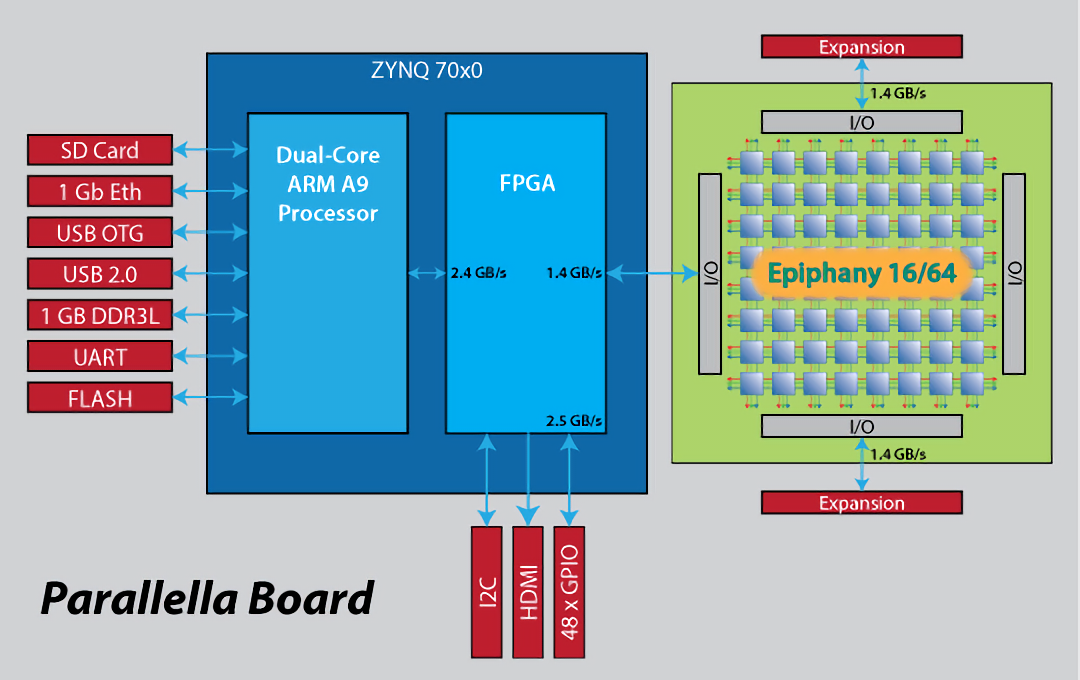
\includegraphics{../images/ParallallaBoardArchitecture.png} 
        }
        \caption{Adapteva Parallella Architecture Overview}
        \label{FIGURE:REQUIRED_KNOWLEDGE_PARALLELA_ARCHITECTURE_OVERVIEW}
    \end{figure}

    \begin{figure}[!ht]
        \centering
        \resizebox{\textwidth}{!}{%
            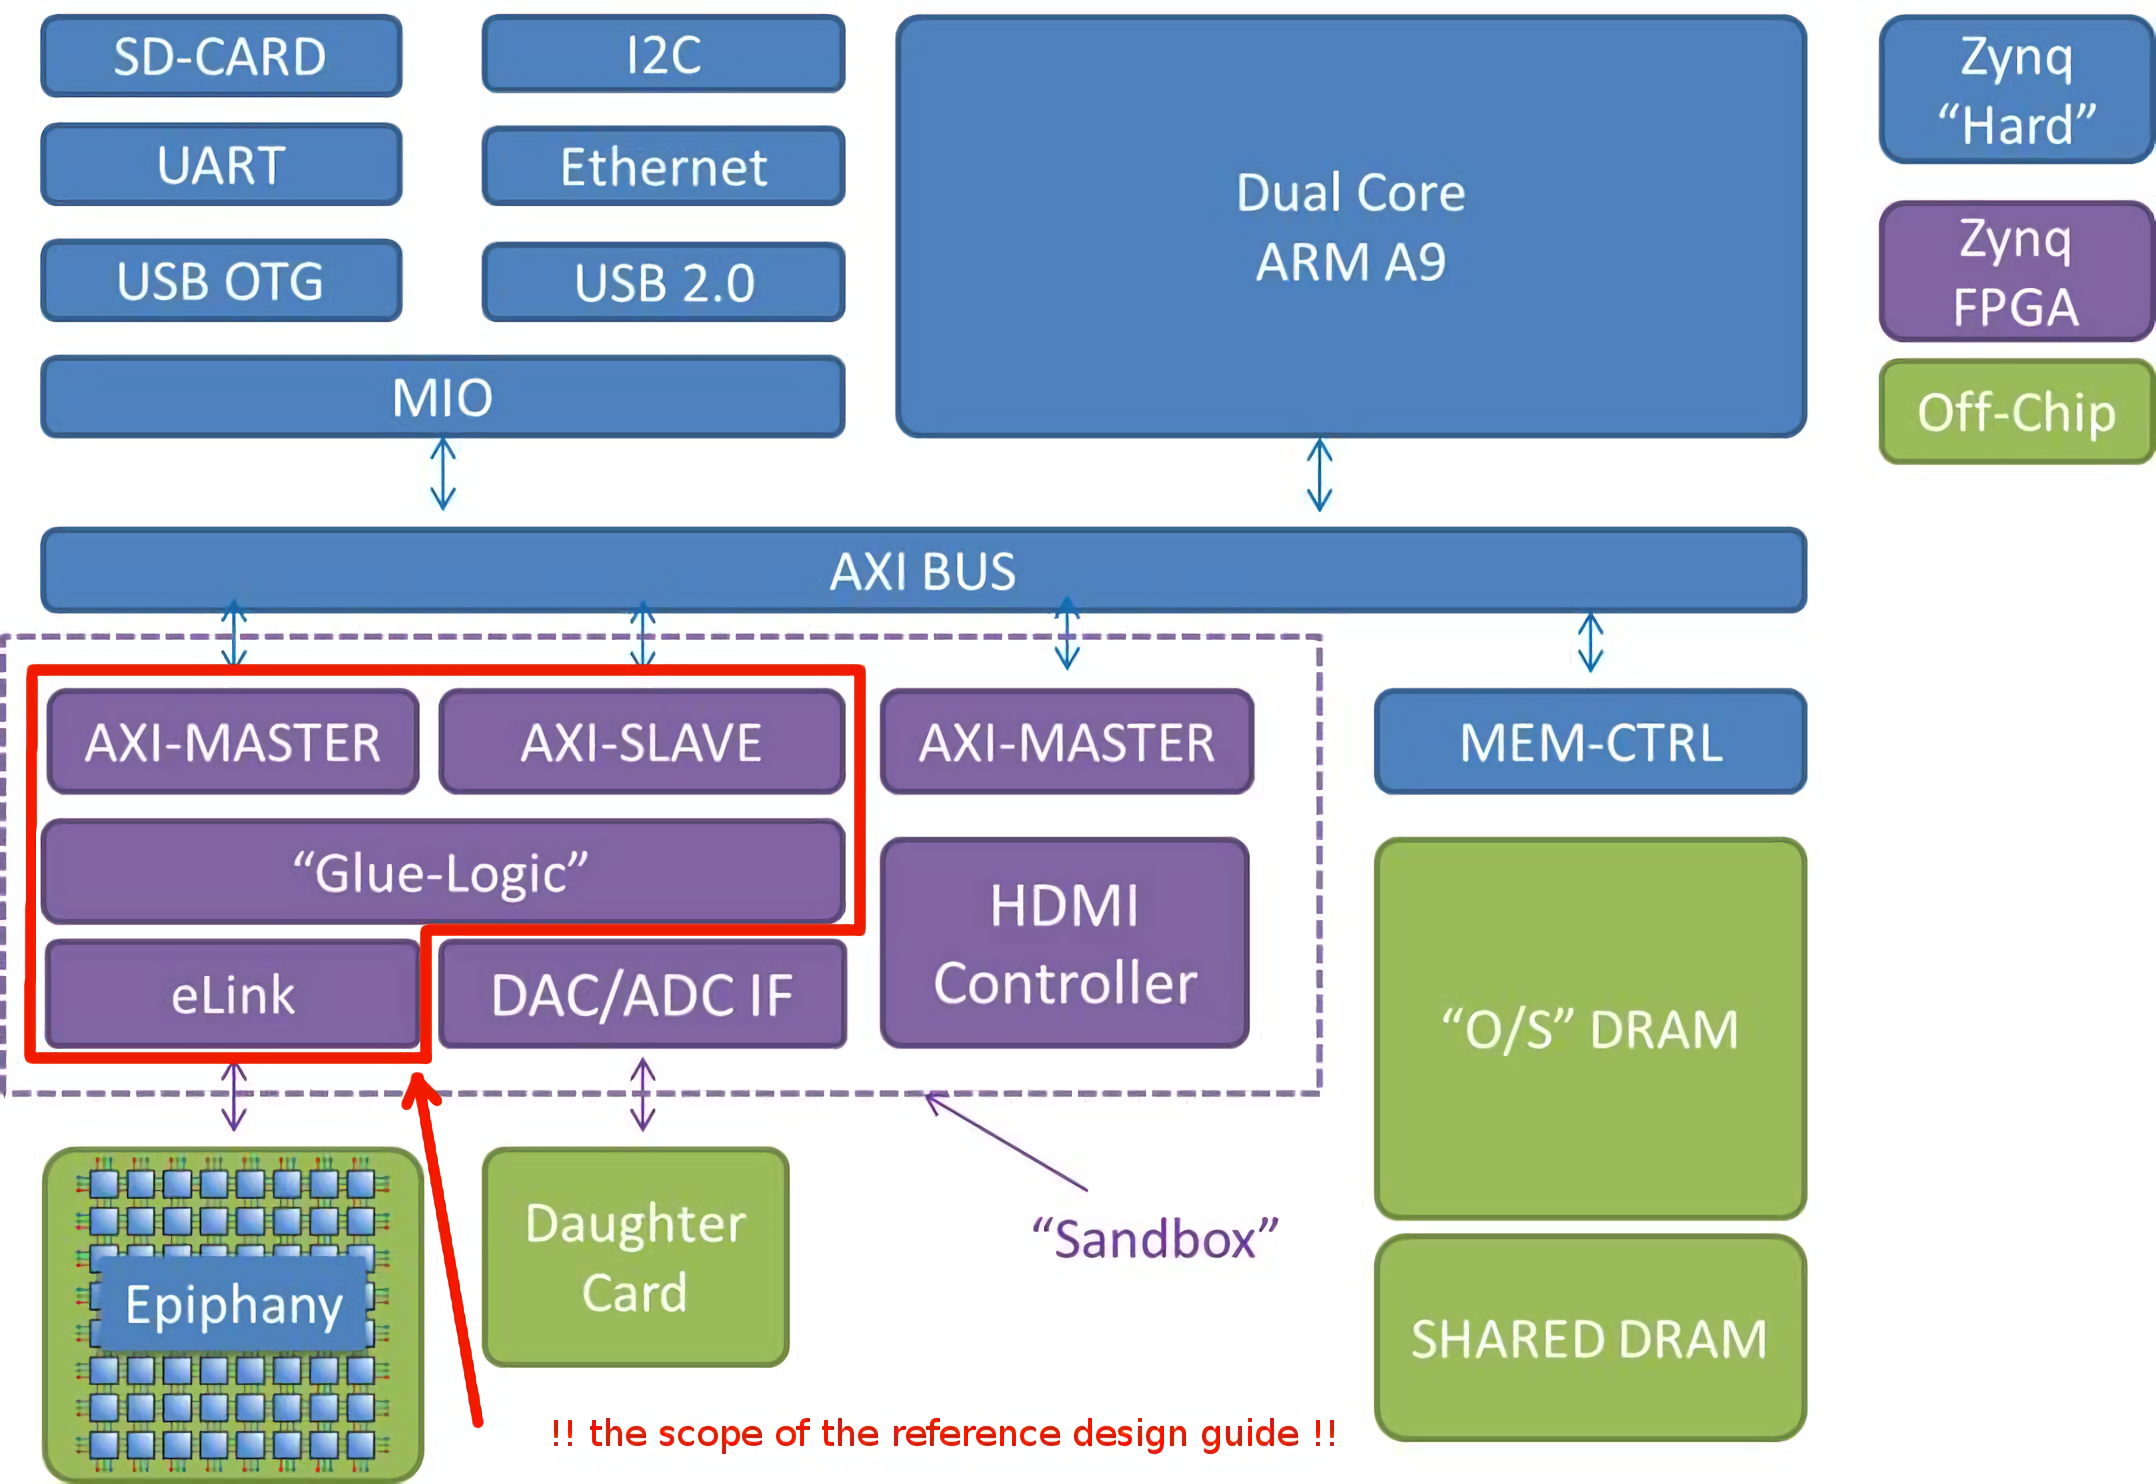
\includegraphics{../images/ParallellaSystem.png} 
        }
        \caption{Adapteva Parallella System Architecture. Physical resources being highlighted in blue, logical resources
        being highlighted in purple and off-chip resources being highlighted in green.}
        \label{FIGURE:REQUIRED_KNOWLEDGE_PARALLELA_SYSTEM_ARCHITECTURE}
    \end{figure}

    \begin{figure}[!ht]
        \centering
        \resizebox{\textwidth}{!}{%
            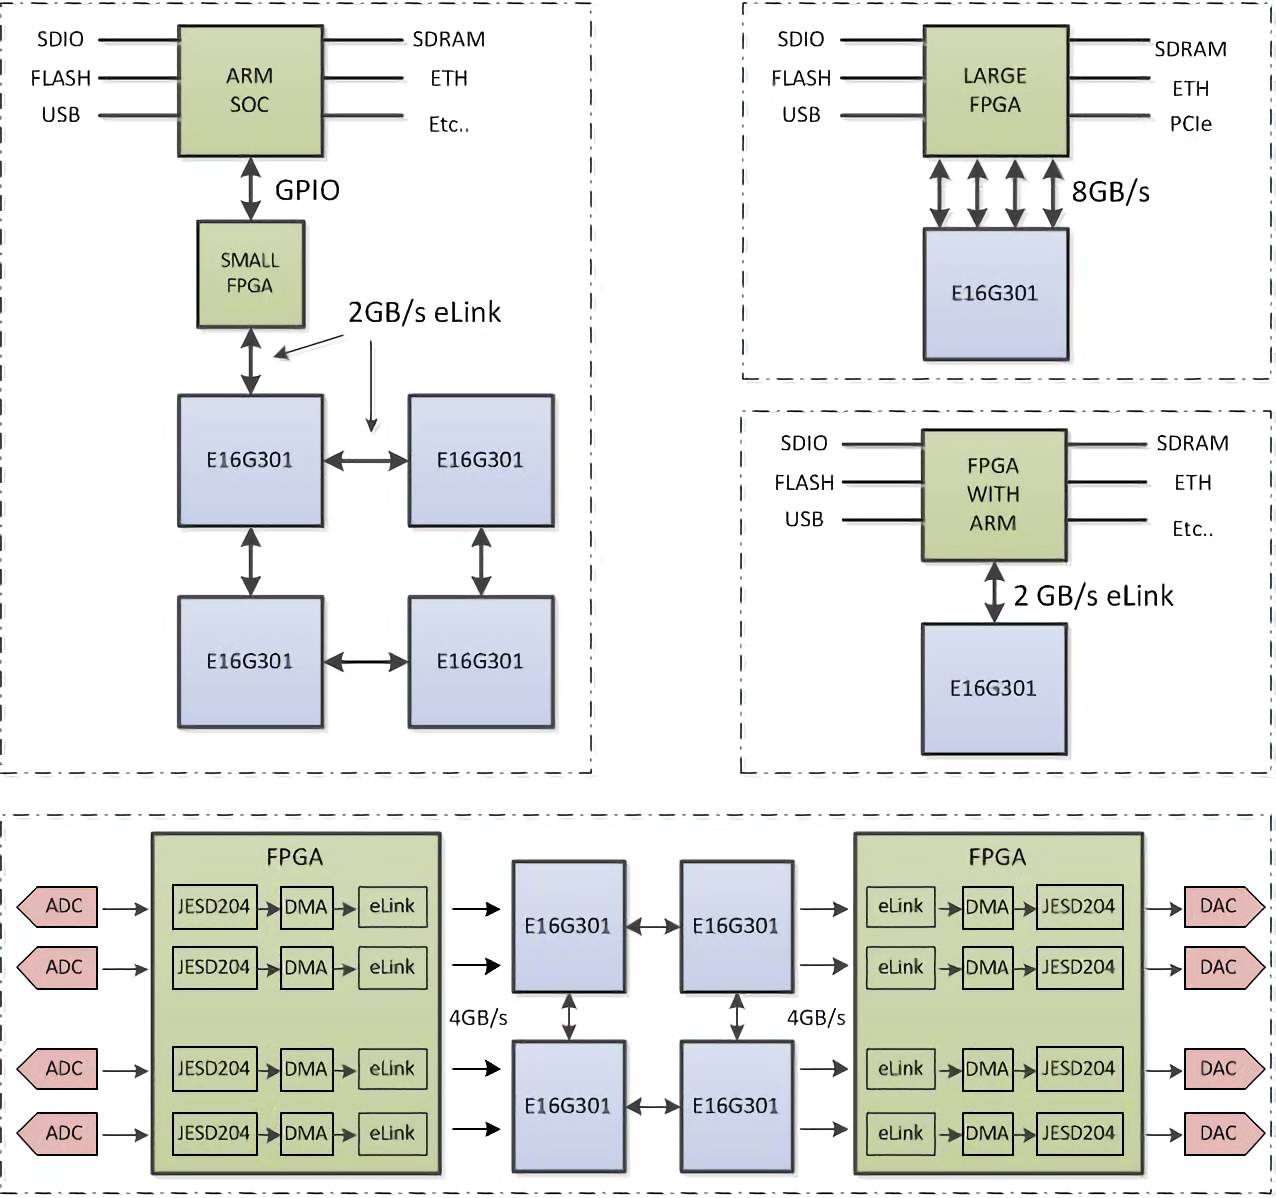
\includegraphics{../images/e16g301system.png} 
        }
        \caption{Adapteva Parallella possible hardware configurations}
        \label{FIGURE:REQUIRED_KNOWLEDGE_PARALLELA_CONFIGURATIONS}
    \end{figure}
